\documentclass{article}
\usepackage[utf8]{inputenc}
\usepackage{graphicx}
\setlength{\parindent}{0pt}
\setlength{\parskip}{1em}

\title{FOAR705 - Learning Journal Week 3}
\author{Jan Jugueta - 44828020}
\date{Week 3: 12/8/19 - 18/8/19}

\begin{document}

\maketitle

\section*{14/8/19 - 1:54pm}

I have continued with the Data Carpentry exercises, resuming with Data Organization in Spreadsheets for Social Scientists. Some general points that stood out to me that I had never considered before were:
\begin{itemize}
    \item Use underscores (\_) instead of spaces when entering data or naming things.
    \item Don’t start naming things with numbers.
    \item Differentiate between a null value and true zero values.
    \item Don’t put multiple tables on the same tab.
    \item Ask yourself if adding a new column to a table will achieve the same result as creating a new tab.
\end{itemize}

\section*{14/8/19 - 2:14pm}

I have revisited the Learn LaTeX in 30 minutes guide and am now going to start with the Scoping Exercise.

\textbf{Overall Objective:} Complete Scoping Exercise using Overleaf and committing the .pdf and .tex file to Cloudstor and the .pdf to iLearn.

\textbf{Objective:} Create new project in Overleaf.

\textbf{Action:} 
\begin{itemize}
    \item Select New Project in Overleaf website.
    \item Name new project ‘Scoping Exercise’
\end{itemize}

\textbf{Error:} None.

\textbf{Result:} New .tex project titled Scoping Exercise in Overleaf.

\section*{14/8/19 - 2:20pm}

\textbf{Objective:} Add title, author name and date to .tex file.

\textbf{Action:}
\begin{itemize}
    \item Changed \begin{verbatim}
        \title{Scoping Exercise} to \title{FOAR705 - Scoping Exercise}    
    \end{verbatim}
    \item Changed \begin{verbatim}
        \author{Jan Jugueta - 44828020}
    \end{verbatim}
    \item Clicked on Recompile to view updated changes.
\end{itemize}

\textbf{Error:} None.

\textbf{Result:} Success. Renamed the default title and author to what I wanted.

\section*{14/8/19 - 2:20pm}

I also note that there is an introduction that is part of the default new project. This is an example of a section in LaTeX. I think I’ll use the sections command to separate the different parts of this assignment.

\textbf{Objective:} Create sections for, Research Area, Jobs, Pains, Pain Relievers, Gains, Gain Creators.

\textbf{Action:}
\begin{itemize}
    \item Changed \begin{verbatim}
        \section{Introduction} to \section{Research Area}
    \end{verbatim}
    \item Added \begin{verbatim}
        \section{Jobs}
    \end{verbatim}
    \item Added \begin{verbatim}
        \section{Pains}
    \end{verbatim}
    \item Added \begin{verbatim}
        \section{Pain Relievers}
    \end{verbatim}
    \item Added \begin{verbatim}
        \section{Gains}
    \end{verbatim}
    \item Added \begin{verbatim}
        \section{Gain Creators}
    \end{verbatim}
    \item Clicked on Recompile to view updated changes.
\end{itemize}

\textbf{Error:} None.

\textbf{Result:} Success. Created all the new sections.

\section*{14/8/19 - 2:40pm}

\textbf{Objective:} See what happens when I start typing text between \begin{verbatim}
    \section{Research Area}
\end{verbatim}
and
\begin{verbatim}
    \section{Jobs}
\end{verbatim}

\textbf{Action:}
\begin{itemize}
    \item Typed a paragraph of information.
    \item Clicked on Recompile to view updated changes.
\end{itemize}

\textbf{Error:} None.

\textbf{Result:} The information I had typed between \begin{verbatim}
    \section{Research Area}
\end{verbatim}
and
\begin{verbatim}
    \section{Jobs} 
\end{verbatim}
appeared as paragraph text in the Research Area section.

\section*{14/8/19 - 2:56pm}

For the Jobs section, I want to experiment with the unordered lists and see how that works with LaTeX. 

\textbf{Objective:} Create a list in LaTeX.

\textbf{Action:}
\begin{itemize}
    \item Using the guide I copied and amended the script provided, and entered this:
    \begin{verbatim}
\begin{itemize}
  \item 
  \item 
  \item 
  \item 
  \item 
  \item 
  \item 
\end{itemize}
    \end{verbatim}
    \item Typed information after every \begin{verbatim}
         \item
    \end{verbatim}
    \item Clicked on Recompile to view updated changes.
\end{itemize}

\textbf{Error:} None.

\textbf{Result:} Dot points have appeared with the text that I have typed in after the \begin{verbatim}
    \item
\end{verbatim}
command.

\section*{14/8/19 - 3:08pm}

For the next section, I want to see how paragraphs work.

\textbf{Objective:} Use paragraphs in the ‘Pains’ section.

\textbf{Action:}
\begin{itemize}
    \item Typed one paragraph underneath the \begin{verbatim}
        \section{Pains}
    \end{verbatim} line.
    \item Created a blank line after that typed paragraph.
    \item Typed a new paragraph after the blank line.
    \item Clicked on Recompile to view updated changes.
\end{itemize}

\textbf{Error:} None.

\textbf{Result:} Separate paragraphs created in the Pains section.

\section*{14/8/19 - 3:41pm}

I have finished filling out the content for my scoping exercise. I will now recompile it, save it and upload both the .tex and .pdf for submission.

\textbf{Objective:} Recompile .tex file and upload files for submission.

\textbf{Action:}
\begin{itemize}
    \item Clicked on recompile.
    \item Reviewed the PDF preview to ensure quality control.
    \item Clicked on Download PDF.
    \item Renamed main.tex to jugueta\_scopingexercise.tex.
    \item Went back to the Project page in Overleaf.
    \item Downloaded jugueta\_scopingexercise.tex.
    \item Opened the Scoping Exercise submission folder in Cloudstor.
    \item Created Jan Jugueta Scoping Exercise in Scoping Exercise submission folder.
    \item Uploaded jugueta\_scopingexercise.tex and Jan\_Jugueta\_Scoping\_Exercise.pdf to  Jan Jugueta Scoping Exercise folder.
    \item Uploaded Jan\_Jugueta\_Scoping\_Exercise.pdf to iLearn.
\end{itemize}

\textbf{Error:} None.

\textbf{Result:} Success. Scoping exercise submitted and uploaded to Cloudstor and iLearn.

\section*{14/8/19 - 4:00pm}

As part of this weeks homework, we were asked to consider problem data produced by our discipline. As I will be mainly work with historical documents, I find that records on sporting tables and match fixtures in East Germany to be wildly inconsistent. I had read the book \textit{The People’s Game}  which is a comprehensive historical account of football in East Germany. However, I had noticed that match records, and how they were display were generally inconsistent for varying seasons. The ‘cells’ in the columns and rows would often contain multiple data sets. Furthermore, they often used special characters to denote more information about a certain data set.

I’m not entirely sure if this example fits the problem data produced by our discipline, but very often, the Stasi (East German Secret Police) would leave lines of information blank when it came to citizens that displayed worrisome anti-socialist behaviours. I would equate this to a null value, which makes me question what information could have been recorded there?

\section*{14/8/19 - 4:10pm}

\textbf{Objective:} Download current version of Learning Journal and commit to GitHub.

\textbf{Action:}
\begin{itemize}
    \item Select File in Cloudstor.
    \item Selected Download As > Docx (Word file).
    \item Downloaded ‘Jan Jugueta - Learning Journal.docx’ to Download Folder on my machine.
    \item Enter Jugueta-Exercises repository in GitHub.
    \item Selected Upload files.
    \item Dragged and dropped ‘Jan Jugueta - Learning Journal.docx’ to upload window in GitHub.
    \item Added the description ‘Learning Journal’.
    \item Added ‘20190814 16:109’ in the extended description to indicate when the Learning Journal was from.
    \item Clicked on Commit changes.
\end{itemize}

\textbf{Error:} None.

\textbf{Result:} Success. Committed Learning Journal to GitHub.

\section*{14/8/19 - 4:11pm}

\textbf{Objective:} Commit Scoping Exercise to GitHub.

\textbf{Action:}
\begin{itemize}
    \item Uploaded Jan\_Jugueta\_Scoping\_Exercise.pdf and jugueta\_scopingexercise.tex to GitHub.
    \item Added ‘Scoping Exercise’ to description.
    \item Added ‘.pdf and .tex’ to extended description.
\end{itemize}

\textbf{Error:} None.

\textbf{Result:} Successfully committed Scoping Exercise to GitHub.

\section*{18/8/19 - 11:41am}

Since I have completed the Scoping Exercise on Overleaf, I have decided to migrate my Learning Journal to Tex as well. So my next step is to transfer my Week 2 Learning Journal to Overleaf.

\textbf{Objective:} Transfer Learning Journal Week 2 to Overleaf.

\textbf{Action:}
\begin{itemize}
    \item Opened new Overleaf Project. 
    \item Titled the project Learning Journal Week 2
    \item Copied and pasted the information from Learning Journal Week 2 from the Cloudstor .docx file into the new Overleaf project.
    \item Used the itemise code to create bullet points where needed.
    \item Click on Recompile.
\end{itemize}

\textbf{Error:} Jan\_JuguetaCV.pdf appeared as Jan_JuguetaCV.pdf.

\textbf{Result:} Copied most of the text successfully, but still need to figure out how to make the underscore '\_' character as an underscore.

\section*{18/8/19 - 12:10pm}

Using the Overleaf guide, I managed to find out the solution to the underscore problem. For underscore to be displayed in normal text, it needs to be preceded by the slash character. 

\textbf{Objective:} Fix the underscore problem in Learning Journal Week 2 in Overleaf.

\textbf{Action:}
\begin{itemize}
    \item Found every instance of where the underscore character appeared and entered the slash character in front of them.
    \item Clicked on recompile.
\end{itemize}

\textbf{Error:} None.

\textbf{Result:} Successfully fixed the underscore problem. They are now displayed as normal text.

\section*{18/8/19 - 12:18pm}

After fixing the underscore problem, I want to figure out how to create a blank vertical space anytime a new paragraph is created. Asking Billy from class, she was able to help me out with the codes:

\begin{itemize}
    \item Entered \begin{verbatim}
        \setlength{\parindent}{0pt}
    \end{verbatim} in the preamble.
    \item Entered \begin{verbatim}
        \setlength{\parskip}{1em} 
    \end{verbatim} in the preamble.
\end{itemize}

\textbf{Error:} None.

\textbf{Result:} Successfully reformatted the .tex file.

\section*{18/8/19 - 12:30pm}

Now that I am happy with the layout of the Learning Journal in Overleaf, I now needed to upload the .tex version of my Learning Journal to Cloudstor and commit a version to GitHub.

\textbf{Objective:} Create a new folder in Cloudstor to store the new .tex Learning Journals. Once done, upload and commit Learning Journals to Cloudstor and GitHub.

\textbf{Action:}
\begin{itemize}
    \item Create new folder in the Learning Journal folder called JuguetaLearningJournal.
    \item Cut and pasted the Jan Jugueta - Learning Journal.docx file into JuguetaLearningJournal Folder.
    \item Downloaded the Learning Journal Week 2 PDF and .tex file from Overleaf.
    \item Created Week2 Folder in JuguetaLearningJournal in Cloudstor.
    \item Uploaded Learning Journal Week 2 .pdf and .tex files into Week2 folder.
    \item Committed the Learning Journal Week 2 .pdf and .tex files into GitHub.
\end{itemize}

\textbf{Error:} None.

\textbf{Result:} Successfully uploaded and committed PDF and Tex files to both Cloudstor and GitHub.

\section*{18/8/19 - 9:20pm}

Started to read the Dates as Data lesson in Data Carpentry. Some important notes here:

\begin{itemize}
    \item Storing dates in a single column is not best practice.
    \item Mac and PC have different dates from when they count their dates.
    \item Excel stores dates as integers.
    \item Regional variances could confuse data.
    \item It is best to record the date as three different data sets ie. Day, Month and Year.
\end{itemize}

\section*{18/8/19 - 9:28pm}

Have downloaded the SAFI\_dates.xlsx file from the Data Carpentry site. To comply with the advice given in earlier Data Carpentry lessons, I will duplicate the sheets to ensure the original data is not modified.

\textbf{Objective:} Create a copy of the DD\_MM\_YEAR tab.

\textbf{Action:}
\begin{itemize}
    \item Right clicked on the DD\_MM\_YEAR tab and selected ‘Move or Copy’.
    \item Selected to create a copy of the DD\_MM\_YEAR tab.
    \item Renamed copied tab DD\_MM\_YEAR\_copy.
\end{itemize}

\textbf{Error:} None.

\textbf{Result:} Success. New copy created.

\section*{18/8/19 - 9:53pm}

Now to create new columns to extract the date data.

\textbf{Objective:} Create columns for the Day, Month and Year.

\textbf{Action:}
\begin{itemize}
    \item Created three new columns.
    \item Entered the text ‘day’, ‘month’ and ‘year’ in the 1st cell of the new columns.
\end{itemize}

\textbf{Error:} None.

\textbf{Result:} Success. Created new columns for day, month and year.

\section*{18/8/19 - 9:57pm}

Now to extract the individual day components from the ‘interview\_date’ column.

\textbf{Objective:} Extract day component from the ‘interview\_date’ column.

\textbf{Action:}
\begin{itemize}
    \item Entered the function =DAY( ) into cell B2.
    \item Recoded the function in cell B2 to =DAY(A2) to reference the ‘interview\_date’ column.
    \item Clicked and dragged the bottom right corner of cell B2 to cell B15 to re-appropriate the =DAY( ) function for their own specific cells.
\end{itemize}

\textbf{Error:} None.

\textbf{Result:} Success. ‘day’ column has extracted the day data from the ‘interview\_date’ column.

\section*{18/8/19 - 10:05pm}

\textbf{Objective:} Extract month component from the ‘interview\_date’ column.

\textbf{Action:}
\begin{itemize}
    \item Entered the function =MONTH( ) into cell C2.
    \item Recoded the function in cell C2 to =MONTH(A2) to reference the ‘interview\_date’ column.
    \item Clicked and dragged the bottom right corner of cell C2 to cell C15 to re-appropriate the =MONTH( ) function for their own specific cells.
\end{itemize}

\textbf{Error:} None.

\textbf{Result:} Success. ‘month’ column has extracted the month data from the ‘interview\_date’ column.

\section*{18/8/19 - 10:11pm}

\textbf{Objective:} Extract year component from the ‘interview\_date’ column.

\textbf{Action:}
\begin{itemize}
    \item Entered the function =YEAR( ) into cell D2.
    \item Recoded the function in cell D2 to =YEAR(A2) to reference the ‘interview\_date’ column.
    \item Clicked and dragged the bottom right corner of cell D2 to cell D15 to re-appropriate the =YEAR( ) function for their own specific cells.
\end{itemize}

\textbf{Error:} None.

\textbf{Result:} Success. ‘year’ column has extracted the year data from the ‘interview\_date’ column.

\section*{18/8/19 - 10:13pm}

Below is a screenshot of the updated SAFI\_dates.xlsx file.

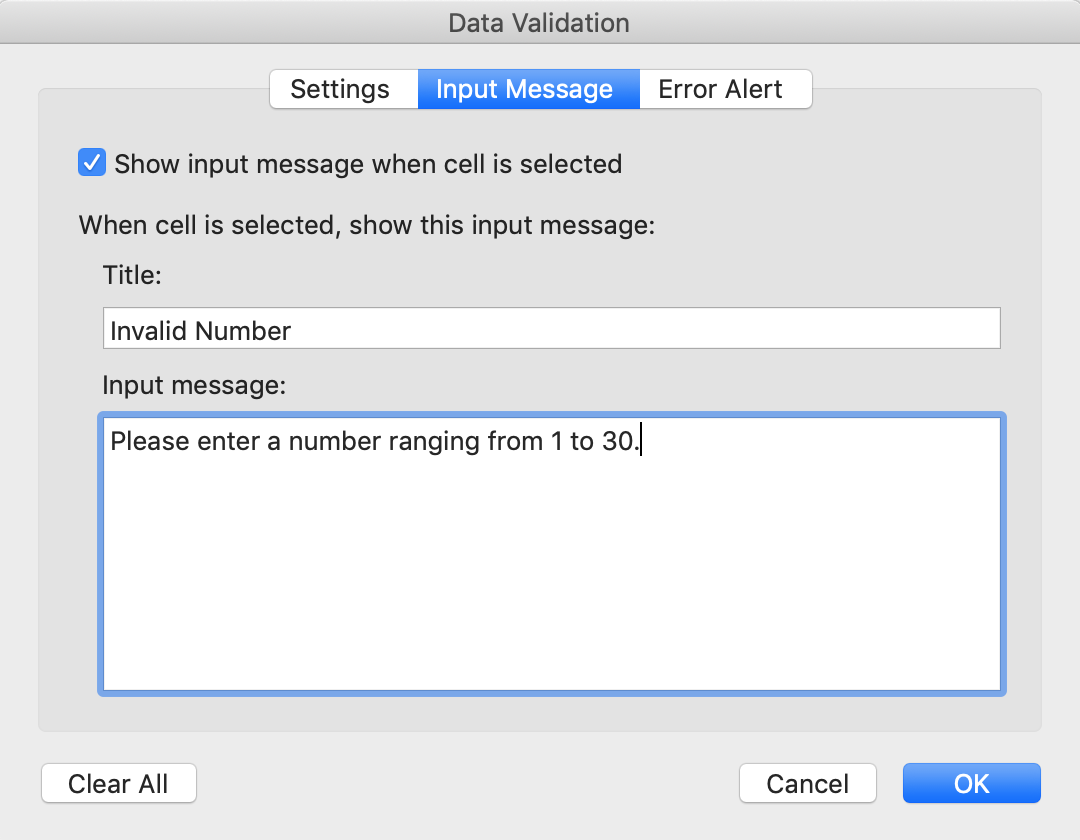
\includegraphics[width=\textwidth]{figa.png}

\section*{18/8/19 - 10:16pm}

Following on to the next section of the exercise. I will now test adding 17/11 to the ‘interview\_date’ column.

\textbf{Objective:} Add 17/11 to interview\_date column.

\textbf{Action:} Entered 17/11 in cell A16.

\textbf{Error:} None.

\textbf{Result:} Cell B16 is displaying 17, cell C16 is displaying 11 and cell D16 is displaying 2019. Thus confirming that if no year data is entered, it will assume that the user implies the current year.

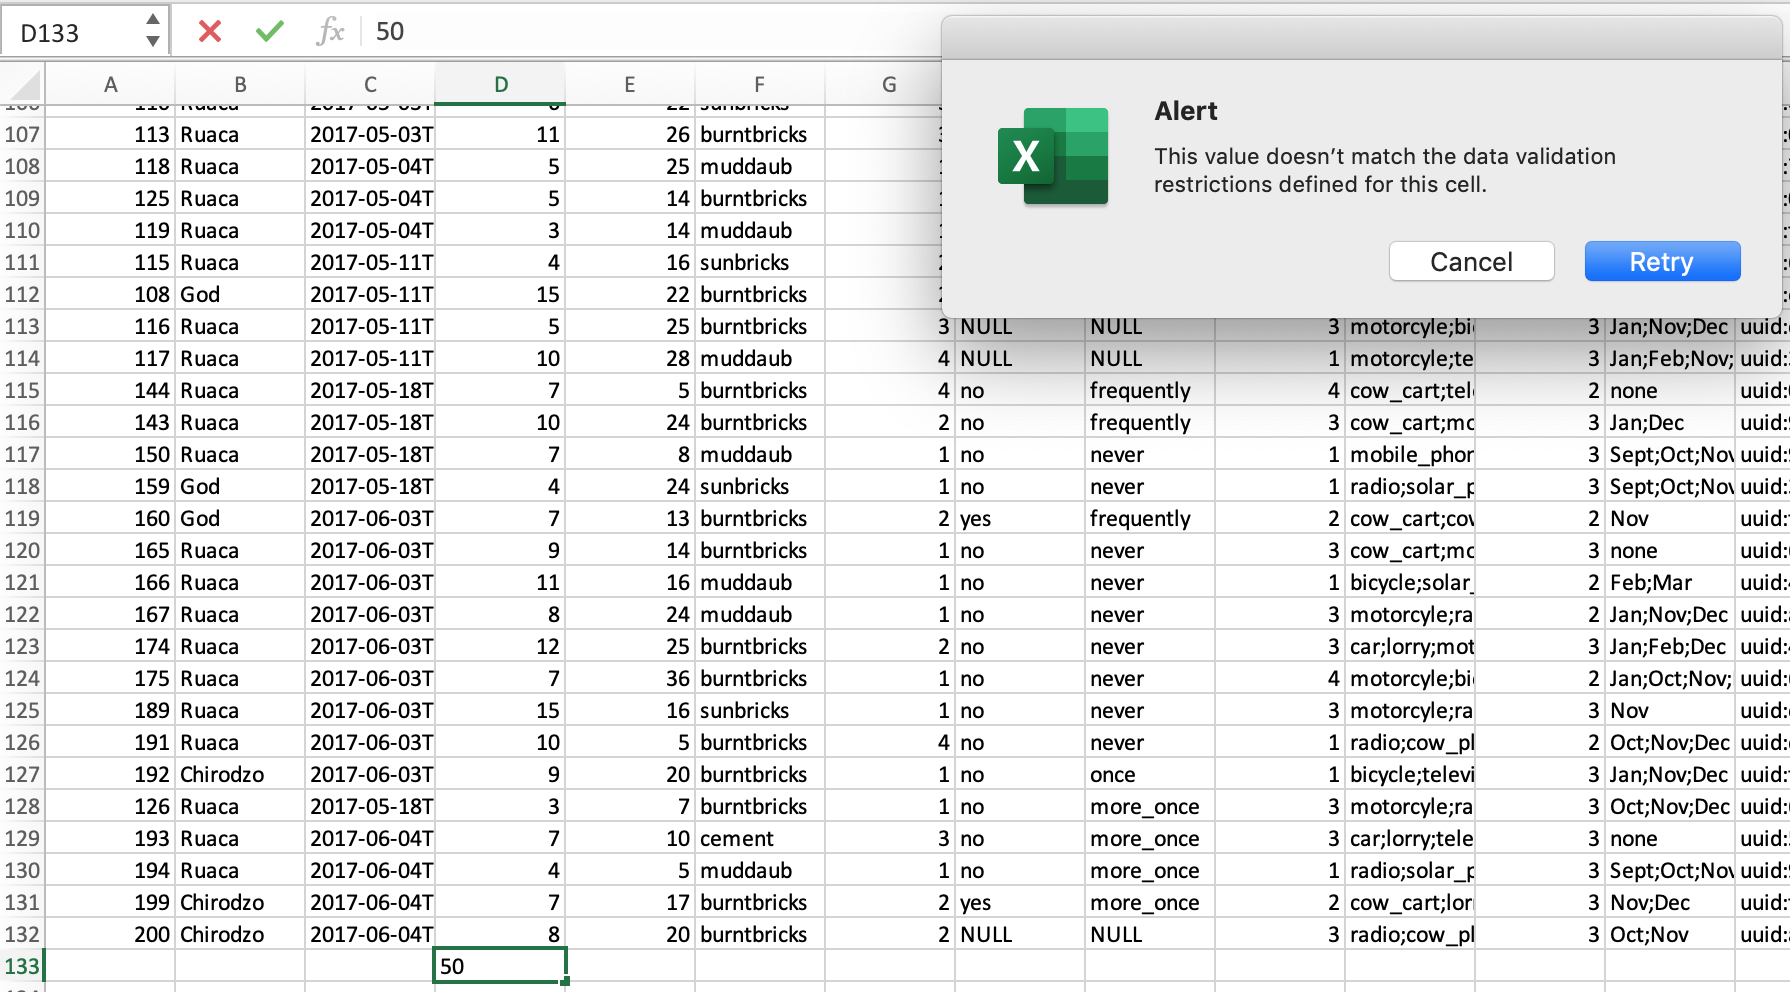
\includegraphics[width=\textwidth]{figb.png}

\section*{18/8/19 - 10:53pm}

Because I want to include screen shots as part of this Learning Journal, I need to learn how to include images in LaTeX.

\textbf{Objective:} Add screenshots to Overleaf and use them in the Journal.

\textbf{Action:}
\begin{itemize}
    \item Uploaded the screenshots to Overleaf.
    \item Renamed the two screenshots to ‘figa.png’ and figb.png’.
    \item Entered \begin{verbatim}
        \usepackage{graphicx}
    \end{verbatim} to the preamble.
    \item Entered the code \begin{verbatim}
        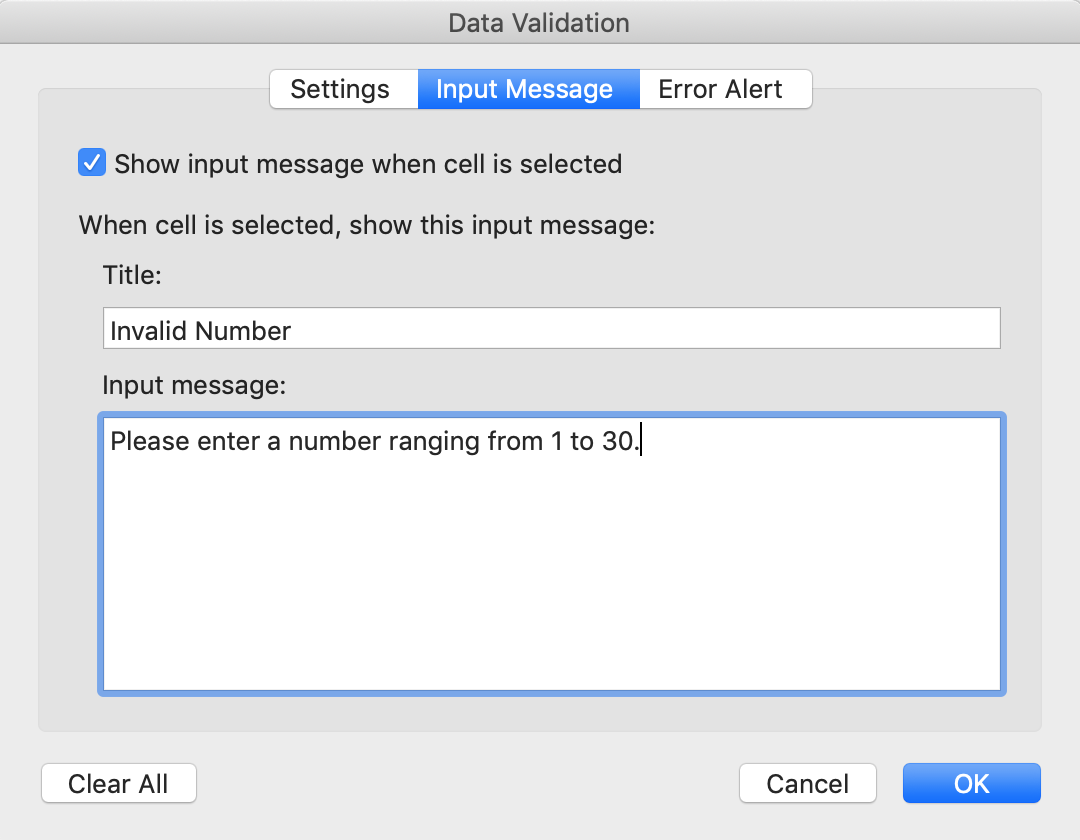
\includegraphics{figa.png}.
    \end{verbatim}
    \item Clicked on recompile to view updated changes.
\end{itemize}

\textbf{Error:} None, but display issues are present.

\textbf{Result:} The image loads, but it is poorly formatted for display.

\section*{18/8/19 - 11:03pm}

I need to resize and position the image so that it fits the page better.

\textbf{Objective:} Resize and position the image for better display.

\textbf{Action:}
\begin{itemize}
    \item Replaced \begin{verbatim}
        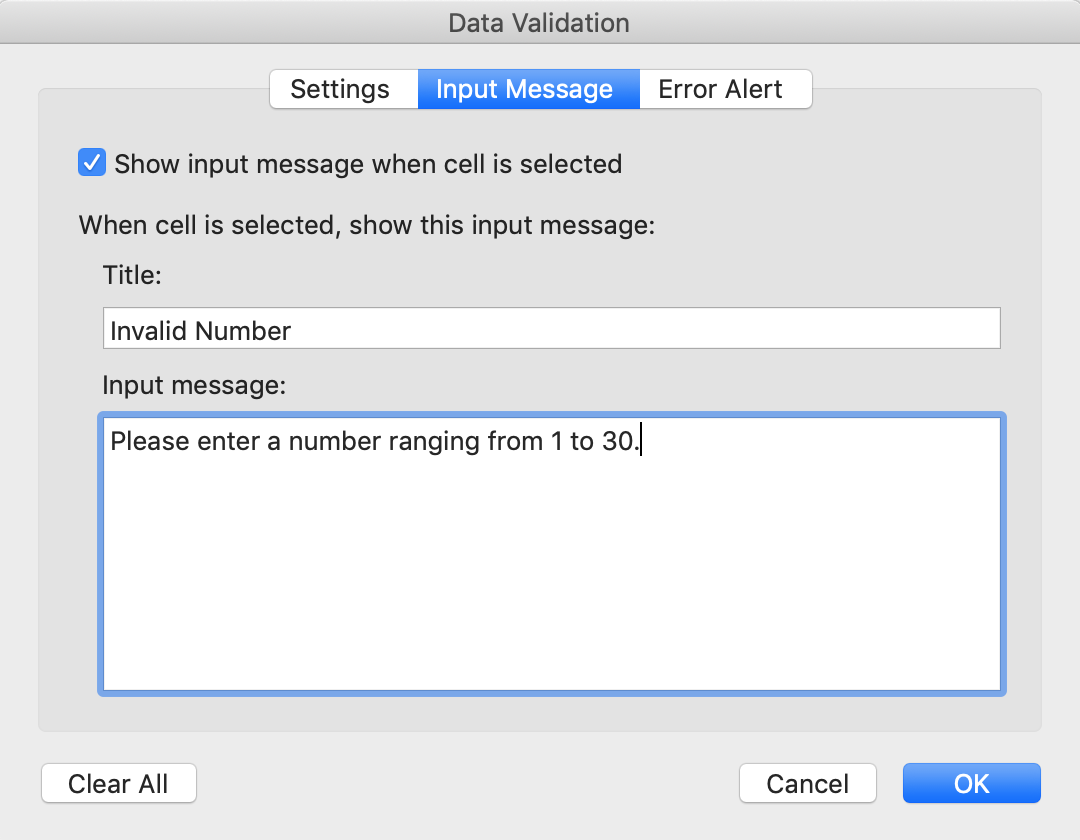
\includegraphics{figa.png}
    \end{verbatim} with
    \begin{verbatim}
        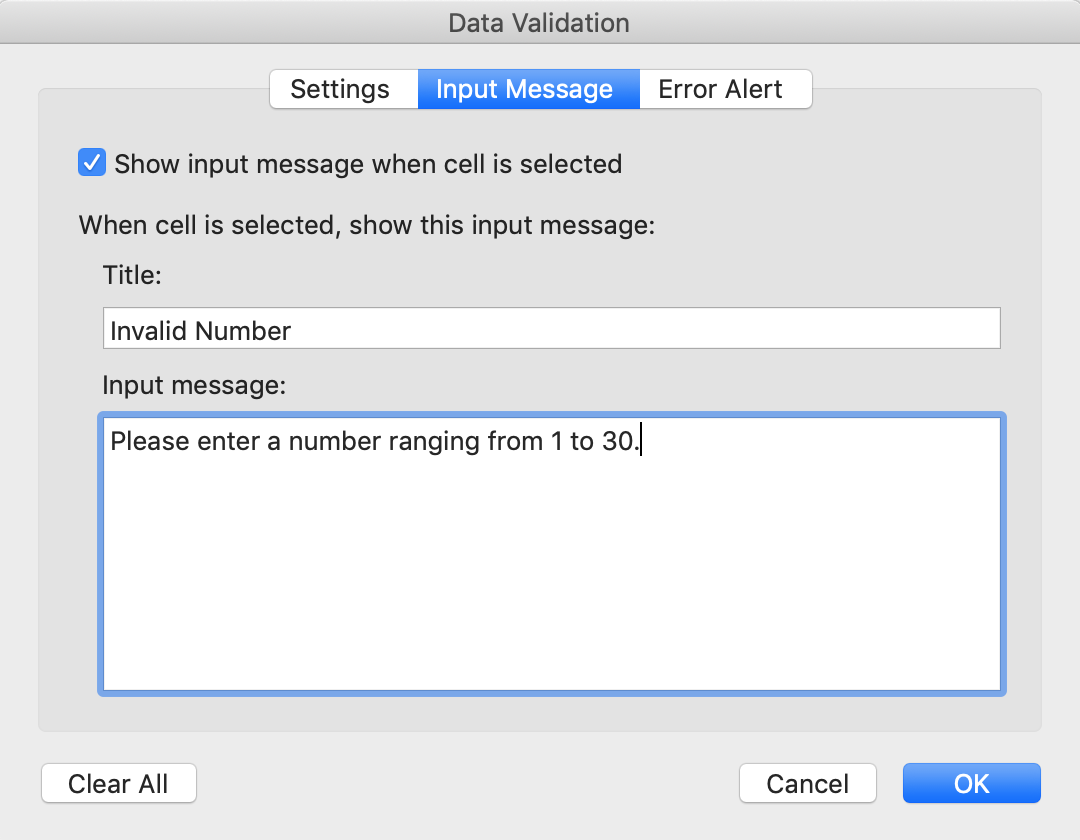
\includegraphics[width=\textwidth]{figa.png}
    \end{verbatim}
    \item Clicked on recompile to view updated changes.
\end{itemize}

\textbf{Error:} None.

\textbf{Result:} Success. Image displayed correctly.

\end{document}
